\documentclass[24pt,pdf,hyperref={unicode}]{beamer}
\usepackage[utf8]{inputenc}
\usepackage{aiml}

\begin{document}

\begin{frame}\frametitle{Аксиомы теории групп}
$\mathcal{G}=(\mathbb{G},\cdot)$

\begin{itemize}
\item<+-> $\forall x,y,z,u\ (x\cdot y=z) \wedge (x\cdot y=u)\rightarrow (z=u)$

\item<+-> $\forall x,y,z\ (x\cdot (y\cdot x))=((x\cdot y)\cdot z) $

\item<+-> $\exists e\forall x\ (x\cdot e)=(e\cdot x)=x$

\item<+-> $\forall x\exists y\ (x\cdot y)=(y \cdot x)=e$
\end{itemize}
\uncover<+->{Доказать единственность единицы:}

\begin{itemize}
\item<+-> $\forall i\ \left[\forall x\ (x\cdot i)=(i\cdot x)=x\right]\rightarrow (e=i)$
\end{itemize}

\uncover<+->{Доказательство}
\begin{itemize}
\item<+-> $(i\cdot e)=i$
\item<+-> $(i\cdot e)=e$
\item<+-> $\therefore e=i$
\end{itemize}
\end{frame}


\begin{frame}\frametitle{Формализация аксиом}
$$
\mathfrak{G}=(\mathbb{G},Eq,G)
$$
$$Eq(x,y)\Leftrightarrow x=y$$
$$G(x,y,z)\Leftrightarrow x\cdot y=z$$

$$
\forall x,y,z,u\ (x\cdot y=z) \wedge (x\cdot y=u)\rightarrow (z=u)
$$
\begin{itemize}
\item<+-> $\forall x \forall y \forall z \forall u\ G(x,y,z) \wedge G(x,y,u)\rightarrow Eq(z,u)$
\item<+-> $\forall x \forall y \forall z \forall u\ \overline{G(x,y,z) \wedge G(x,y,u)}\vee Eq(z,u)$
\item<+-> $\forall x \forall y \forall z \forall u\ \neg G(x,y,z) \vee \neg G(x,y,u)\vee Eq(z,u)$
\item<+-> $G(x,y,z) \vee \neg G(x,y,u)\vee Eq(z,u)$
\end{itemize}
\end{frame}

\begin{frame}\frametitle{Формализация аксиом}
$$
\exists e\forall x\ (x\cdot e)=(e\cdot x)=x
$$
\begin{itemize}
\item<+-> $\exists e\forall x\ G(x,e,x)\wedge G(e,x,x)$
\item<+-> $G(x,e,x)\wedge G(e,x,x)$
\item<+-> $G(t,e,t),\ G(e,t,t)$
\end{itemize}
\end{frame}

\begin{frame}\frametitle{Формализация теоремы}
$$
\forall i\ \left[\forall x\ (x\cdot i)=(i\cdot x)=x\right]\rightarrow (e=i)
$$
\begin{itemize}
\item<+-> $\forall i\ \left[\forall x\ G(x,i,x)\wedge G(i,x,x) \right]\rightarrow Eq(e,i)$
\item<+-> $\overline{\forall i\ \left[\forall x\ G(x,i,x)\wedge G(i,x,x) \right]\rightarrow Eq(e,i)}$
\item<+-> $\overline{\forall i\ \overline{\left[\forall x\ G(x,i,x)\wedge G(i,x,x) \right]}\vee Eq(e,i)}$
\item<+-> $\exists i\ \overline{\overline{\left[\forall x\ G(x,i,x)\wedge G(i,x,x) \right]}\vee Eq(e,i)}$
\item<+-> $\exists i\ \overline{\overline{\left[\forall x\ G(x,i,x)\wedge G(i,x,x) \right]}}\wedge \neg Eq(e,i)$
\item<+-> $\exists i\ \left[\forall x\ G(x,i,x)\wedge G(i,x,x) \right]\wedge \neg Eq(e,i)$
\item<+-> $\exists i\forall x\  G(x,i,x)\wedge G(i,x,x) \neg Eq(e,i)$
\item<+-> $G(x,i,x)\wedge G(i,x,x) \wedge \neg Eq(e,i)$
\item<+-> $G(s,i,s),\ G(i,s,s),\ \neg Eq(e,i)$
\end{itemize}
\end{frame}

\begin{frame}\frametitle{Доказательство теоремы}

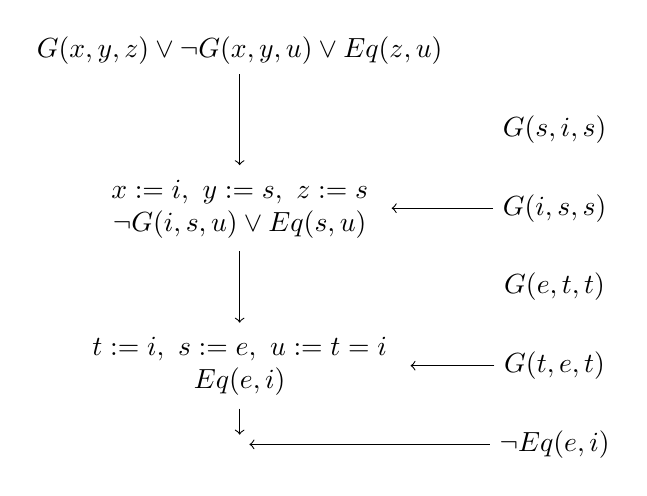
\begin{tikzpicture}

\node (eq) at (0,5) {$G(x,y,z) \vee \neg G(x,y,u)\vee Eq(z,u)$};
\node (i1) at (4,4) {$G(s,i,s)$};
\node (i2) at (4,3) {$G(i,s,s)$};
\node (e2) at (4,2) {$G(e,t,t)$};
\node (e1) at (4,1) {$G(t,e,t)$};
\node (neq) at (4,0) {$\neg Eq(e,i)$};

\uncover<+->{
\node(s1) at (0,3) {$\begin{array}{c}x:=i,\ y:=s,\ z:=s\\ \neg G(i,s,u)\vee Eq(s,u)\end{array}$};
\path (eq) edge[->] (s1);
\path (i2) edge[->] (s1);
}

\uncover<+->{
\node(s2) at (0,1) {$\begin{array}{c}t:=i,\ s:=e,\ u:=t=i\\  Eq(e,i)\end{array}$};
\path (e1) edge[->] (s2);
\path (s1) edge[->] (s2);
}

\uncover<+->{
\node(s3) at (0,0) {$\square$};
\path (s2) edge[->] (s3);
\path (neq) edge[->] (s3);
}
\end{tikzpicture}
\end{frame}

\begin{frame}\frametitle{Поиск теоремы}
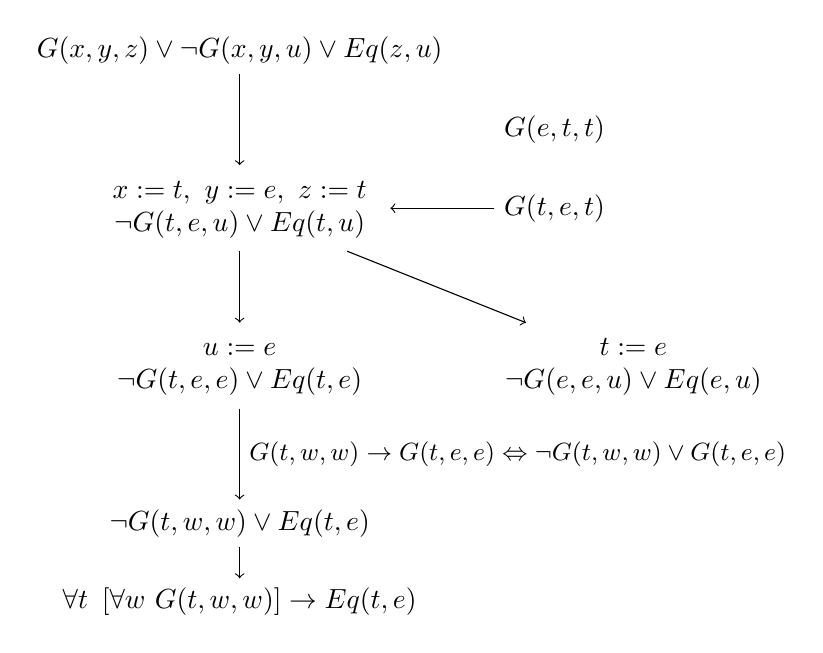
\begin{tikzpicture}
\node (eq) at (0,5) {$G(x,y,z) \vee \neg G(x,y,u)\vee Eq(z,u)$};
\node (e2) at (4,4) {$G(e,t,t)$};
\node (e1) at (4,3) {$G(t,e,t)$};


\uncover<2->{
\node(s1) at (0,3) {$\begin{array}{c}x:=t,\ y:=e,\ z:=t\\ \neg G(t,e,u)\vee Eq(t,u)\end{array}$};
\path (eq) edge[->] (s1);
\path (e1) edge[->] (s1);
}

\uncover<3->{
\node(s2) at (0,1) {$\begin{array}{c}u:=e \\ \neg G(t,e,e)\vee Eq(t,e)\end{array}$};
\path (s1) edge[->] (s2);
}

\only<4>{
\node(s3) at (5,1) {$\begin{array}{c}t:=e \\ \neg G(e,e,u)\vee Eq(e,u)\end{array}$};
\path (s1) edge[->] (s3);
}

\uncover<5->{
\node(s3) at (0,-1) {$\neg G(t,w,w)\vee Eq(t,e)$};
\path (s2) edge[->] node[right]{\small $G(t,w,w)\rightarrow G(t,e,e)\Leftrightarrow \neg G(t,w,w)\vee G(t,e,e)$} (s3);
}

\uncover<6->{
\node(s4) at (0,-2) {$\forall t\ \left[\forall w\ G(t,w,w)\right]\rightarrow Eq(t,e)$};
\path (s3) edge[->] (s4);
}


\end{tikzpicture}
\end{frame}

\begin{frame}\frametitle{Robbin's conjecture}
$$
\begin{array}{l l}
& (A\vee B)\vee C = A \vee (B\vee C) \\
& A\vee B=B\vee A \\
& \neg( \neg(A\vee B) \vee \neg(A\vee \neg B) ) = A\\
\hline 
\therefore & \neg \neg A=A
\end{array}
$$
\end{frame}
\end{document}
